\documentclass[UTF8]{article}
\usepackage{graphicx}
\usepackage{CJK}
\usepackage{epstopdf}
\begin{document}
\begin{CJK}{UTF8}{gkai}
\title{数字信号处理实验报告}
\author{杨庆龙\quad 1500012956\\yangqinglong@pku.edu.cn}
\date{2018.4}
\maketitle

\section{实验一}
问题描述:有限长序列x(n)=[0,3,5,7,9,8,1,2,4,6],按要求完成以下各小题
\subsection{求出它的DFT,请画出对应的幅度谱和相位谱;}
考虑到Matlab适合用于矩阵运算而非C语言式的下标寻址运算,所以考虑使用DFT的矩阵算法,即公式\ref{pro1_1}。
\begin{equation}
\left[\begin{array}{c}
X(0)\\
X(1)\\
\vdots\\
X(N-1)
\end{array}\right]
=
\left[\begin{array}{cccc}
1 & 1 & \cdots & 1\\
1 & W_N^1 \cdots & W_N^{N-1}\\
\vdots&\vdots&\ddots&\vdots\\
1 & W_N^{N-1} & \cdots & W_N^{(N-1)(N-1)}
\end{array}
\right]
\left[
\begin{array}{c}
  x(0)\\
  x(1)\\
  \vdots\\
  x(N-1)
\end{array}
\right]\label{pro1_1}
\end{equation}
观察公式\ref{pro1_1}中的DFT矩阵可得,该矩阵中的指数矩阵可由公式\ref{pro1_2}算出。
\begin{equation}
  \left[\begin{array}{cccc}
  0&0&\cdots&0\\
  0&1&\cdots&N-1\\
  \vdots&\vdots&\ddots&\vdots\\
  0&N-1&\cdots&(N-1)(N-1)
  \end{array}
  \right]
  =
  \left[\begin{array}{c}
  0\\
  1\\
  \vdots\\
  N-1
  \end{array}
  \right]
  \left[\begin{array}{cccc}
  0&1&\cdots&N-1
  \end{array}
  \right]\label{pro1_2}
\end{equation}
因此,该DFT算法流程为
\begin{enumerate}
  \item 求出输入向量长度
  \item 得到N维向量
  \item 求出指数矩阵
  \item 求出DFT矩阵
  \item 求出DFT结果
\end{enumerate}
算法运行结果如图\ref{pro1_fig1}
\begin{figure}
  \centering
  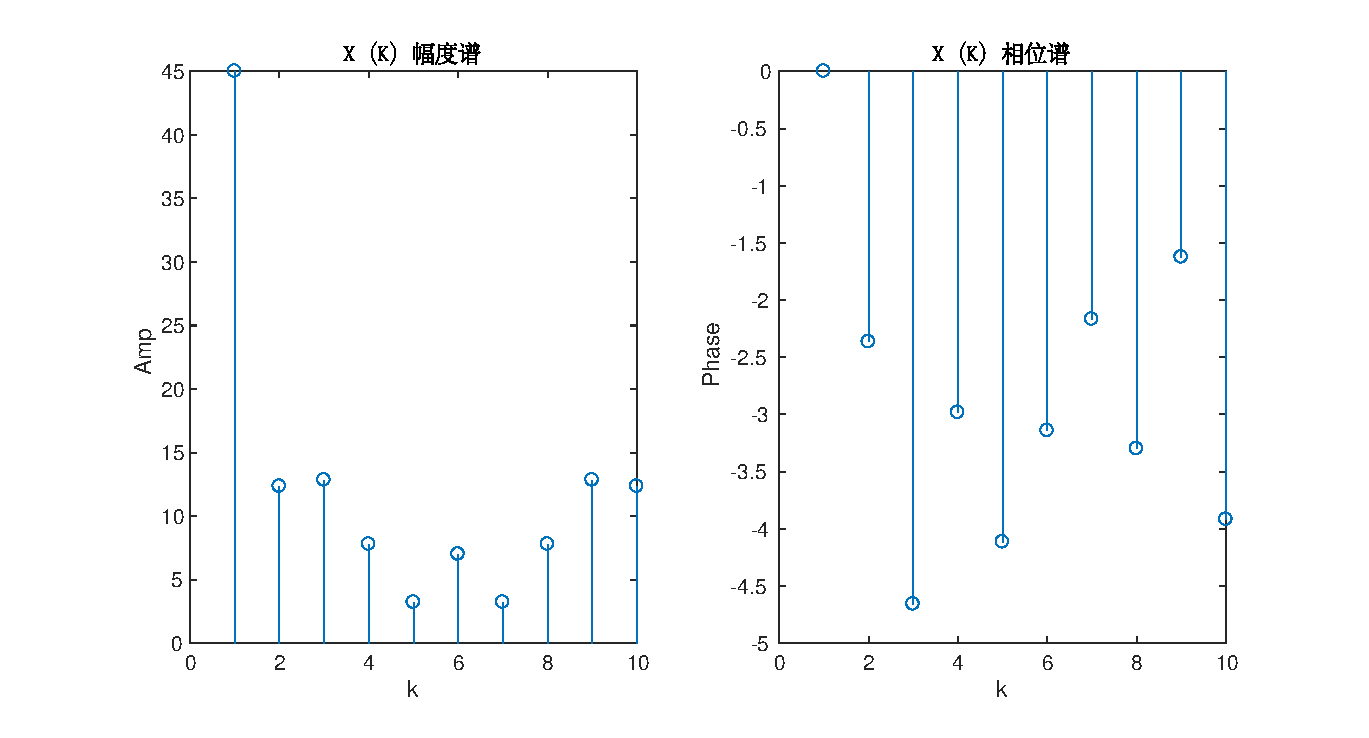
\includegraphics[scale=0.3]{pro1_subpro1.eps}
  \caption{输入信号DFT输出结果图}
  \label{pro1_fig1}
\end{figure}

\subsection{求它的IDFT,画出原信号与IDFT信号的对比图}
IDFT一样有矩阵算法,即公式\ref{pro1_3}
\begin{equation}
\left[\begin{array}{c}
x(0)\\
x(1)\\
\vdots\\
x(N-1)
\end{array}\right]
=
\frac{1}{N}
\left[\begin{array}{cccc}
1 & 1 & \cdots & 1\\
1 & W_N^{-1} \cdots & W_N^{-(N-1)}\\
\vdots&\vdots&\ddots&\vdots\\
1 & W_N^{-(N-1)} & \cdots & W_N^{-(N-1)(N-1)}
\end{array}
\right]
\left[
\begin{array}{c}
  X(0)\\
  X(1)\\
  \vdots\\
  X(N-1)
\end{array}
\right]\label{pro1_3}
\end{equation}
观察得出,其与DFT算法类似,只是指数矩阵需要求相反数,再乘上归一化常数即可。故此处不再赘述。IDFT结果如图\ref{pro1_fig2}和图\ref{pro1_fig3}。从图中可以看出,原信号和IDFT得到的信号不论是幅度,还是相位都相同,这也才符合DFT的基本要求。
\begin{figure}
  \centering
  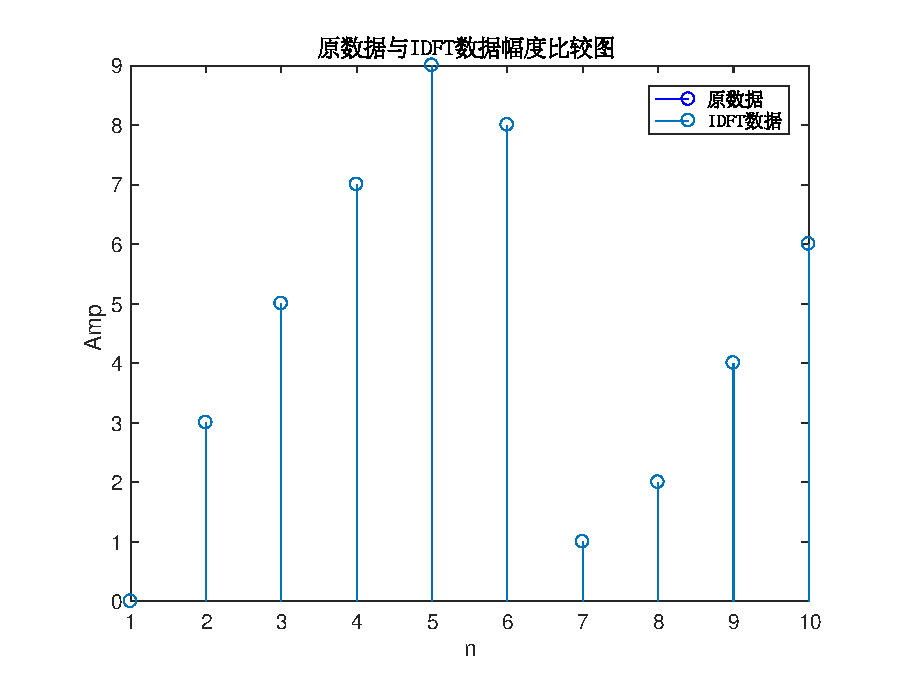
\includegraphics[scale=0.5]{pro1_subpro2_amp.eps}
  \caption{IDFT结果与原信号幅度对比图}
  \label{pro1_fig2}
\end{figure}
\begin{figure}
  \centering
  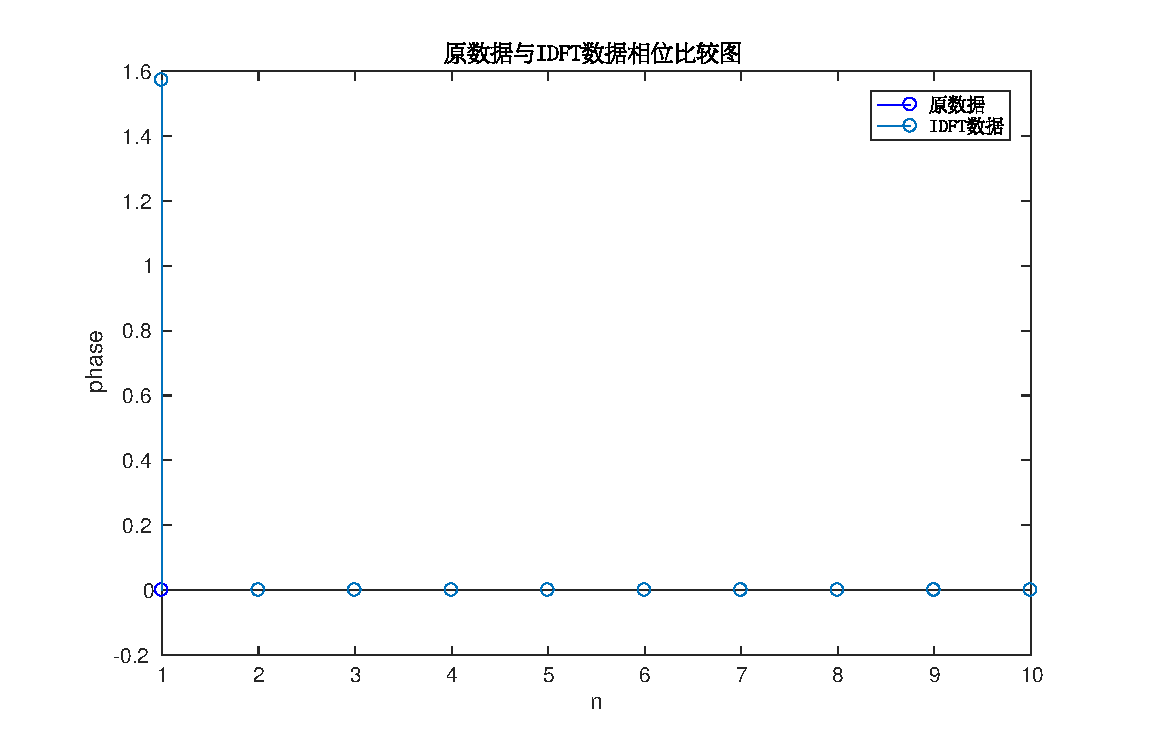
\includegraphics[scale=0.5]{pro1_subpro2_phase.eps}
  \caption{IDFT结果与原信号幅度对比图}
  \label{pro1_fig3}
\end{figure}
\subsection{在x(n)后面分别补10个0, 990个0,求新序列的DFT,并与原序列进行比较,解释不同}
按照题目要求,补0后再进行DFT运算得到的结果如图\ref{pro1_fig4}。从图中可以看出,对于幅度谱来说,补0后可以得到更高的分辨率,补的0越多分辨率越高,而不补0得到的结果也只是在补了很多0之后等间隔采样,最多也只是最后一个点因为函数连续性的问题而偏差较大,但也足够在相当的程度上反应该信号的幅度谱。\\
但对于相位谱却并不是如此,很容易可以看到,即使只是补了10个0的相位谱也已经和补了990个0的相位谱差别不大。然而不补0的序列DFT得到的相位谱却与之相差极大,这是因为相位具有每$2\pi$循环一周的特点,所以DFT求出的相邻两点间的相位差一直都位于$[-\pi,\pi]$的范围内。所以当频域采样间隔不够时,计算得到的结果就会将原本相位相差很多个$\pi$的结果取余数至$[-\pi,\pi]$也就不能反映真实的相位变化情况。因此,对于需要考虑某个信号相位谱的情况,必须进行补0操作再DFT,否则将无法合理判断出同相点和反相点所在位置。
\begin{figure}
  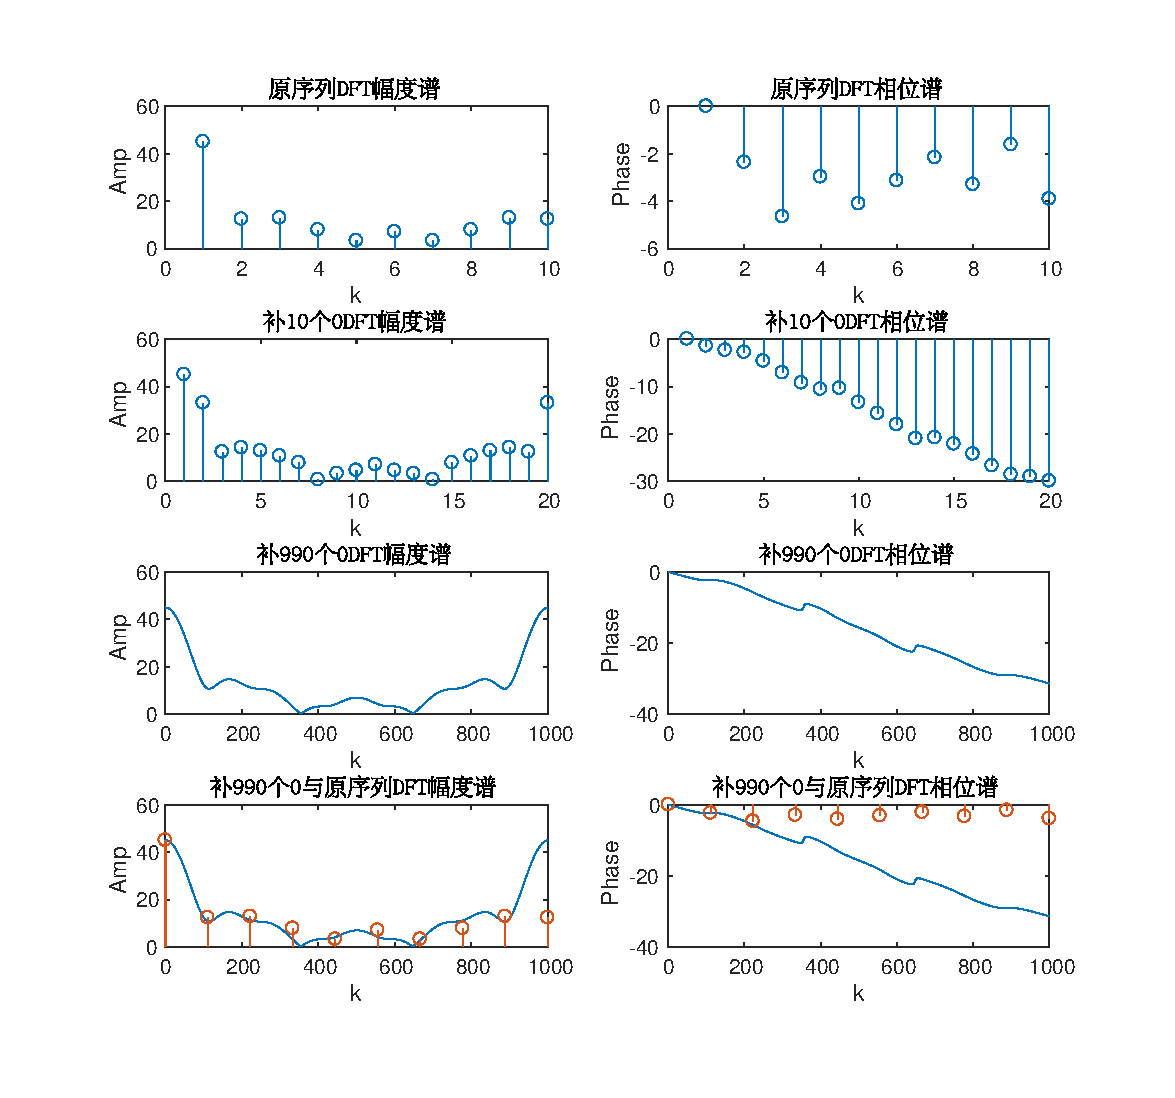
\includegraphics[scale=0.5]{pro1_subpro3.eps}
  \caption{序列补0DFT结果比较图}
  \label{pro1_fig4}
\end{figure}
\subsection{对x(n)进行8倍上采样(即每个点后面补7个0),求其DFT,并与原序列进行比较,解释不同}
为了实现起来比较简单,所以直接使用Matlab自带的upsample函数进行上采样操作,采样倍数选择8即可满足题目要求。再进行DFT计算后得到的结果如图\ref{pro1_fig5}和图\ref{pro1_fig6}。从这两幅图中可以看出,上采样后幅度谱被重复了8次 ,这使得噪声被平均分配到这八个谱上,然而我们只需要其中一个谱即可。所以这可以将噪声对传输的干扰减小到原来的$\frac{1}{8}$,极大地改善了传输效果。\\
观察相位谱可以发现,该相位谱也只是在周期重复,但由于DFT的相位差只能位于$[-\pi,\pi]$的范围内,所以出现了每重复一次相位差增加一个$2\pi$的情况,但又考虑到恢复信号的时候,相位谱不但只取八个谱中的一个,还要对$2\pi$取余,所以这些多出来的相位并不会对结果产生影响。\\
综上,八倍上采样可以将噪声对幅度谱和相位谱的影响都降低到原来的$\frac{1}{8}$,提高通信的质量。
\begin{figure}
  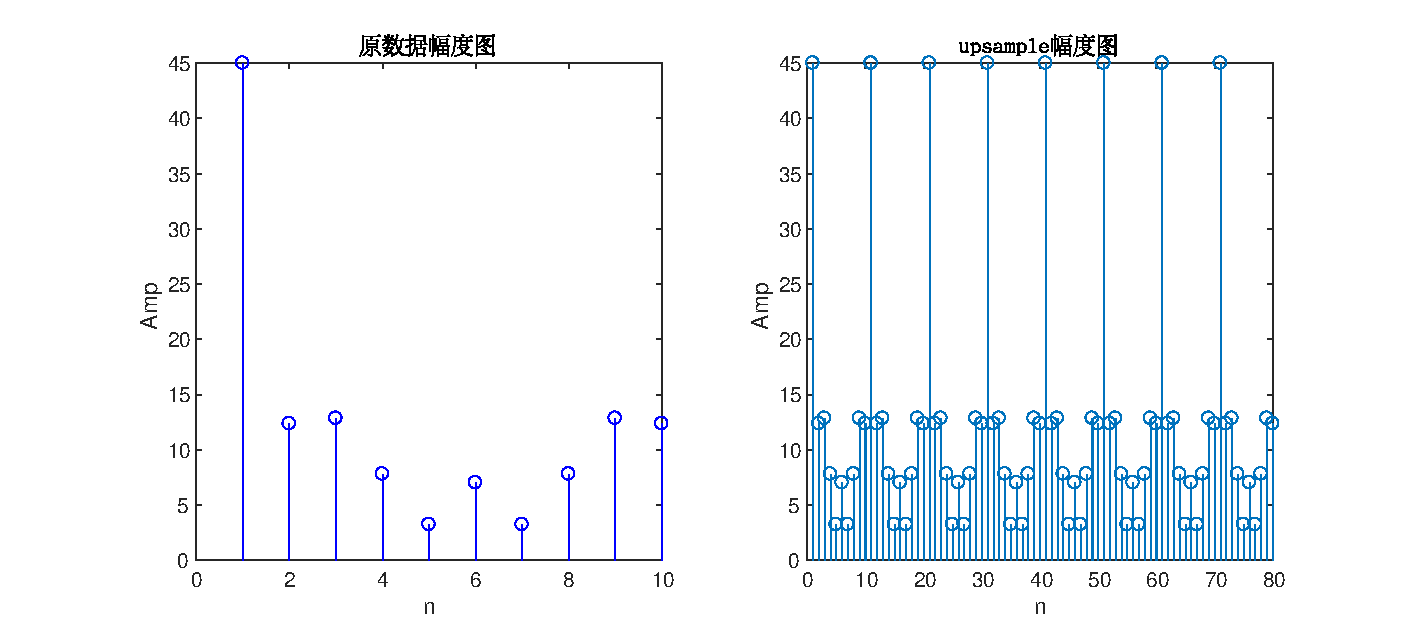
\includegraphics[scale=0.4]{pro1_subpro4_amp.eps}
  \caption{八倍上采样后的幅度谱}
  \label{pro1_fig5}
\end{figure}

\begin{figure}
  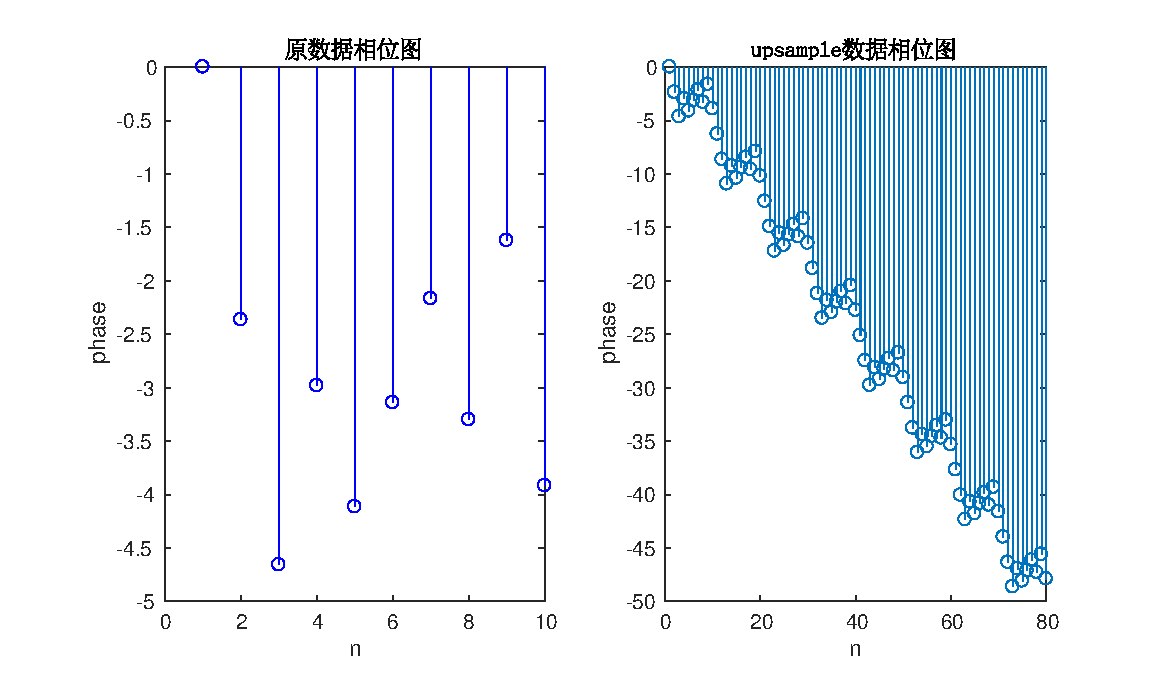
\includegraphics[scale=0.4]{pro1_subpro4_phase.eps}
  \caption{八倍上采样后相位谱}
  \label{pro1_fig6}
\end{figure}
\section{实验二}
问题描述:模拟信号$x_a=\sin(2\pi f_0t)+0.5\sin(6\pi f_0t),f_0=1Hz$,按要求完成以下各小题:
\subsection{分别设定采样频率为$5f_0$、$10f_0$、$15f_0$,绘制模拟信号图和采样后的离散信号图;(只需画出三个周期即可t:0—3)}
先生成采样间隔$1000f_0$的时间序列模拟出模拟信号的时域波形,再分别生成所需采样间隔的时间序列进行采样。得到的结果如图\ref{pro2_fig1}
\begin{figure}
  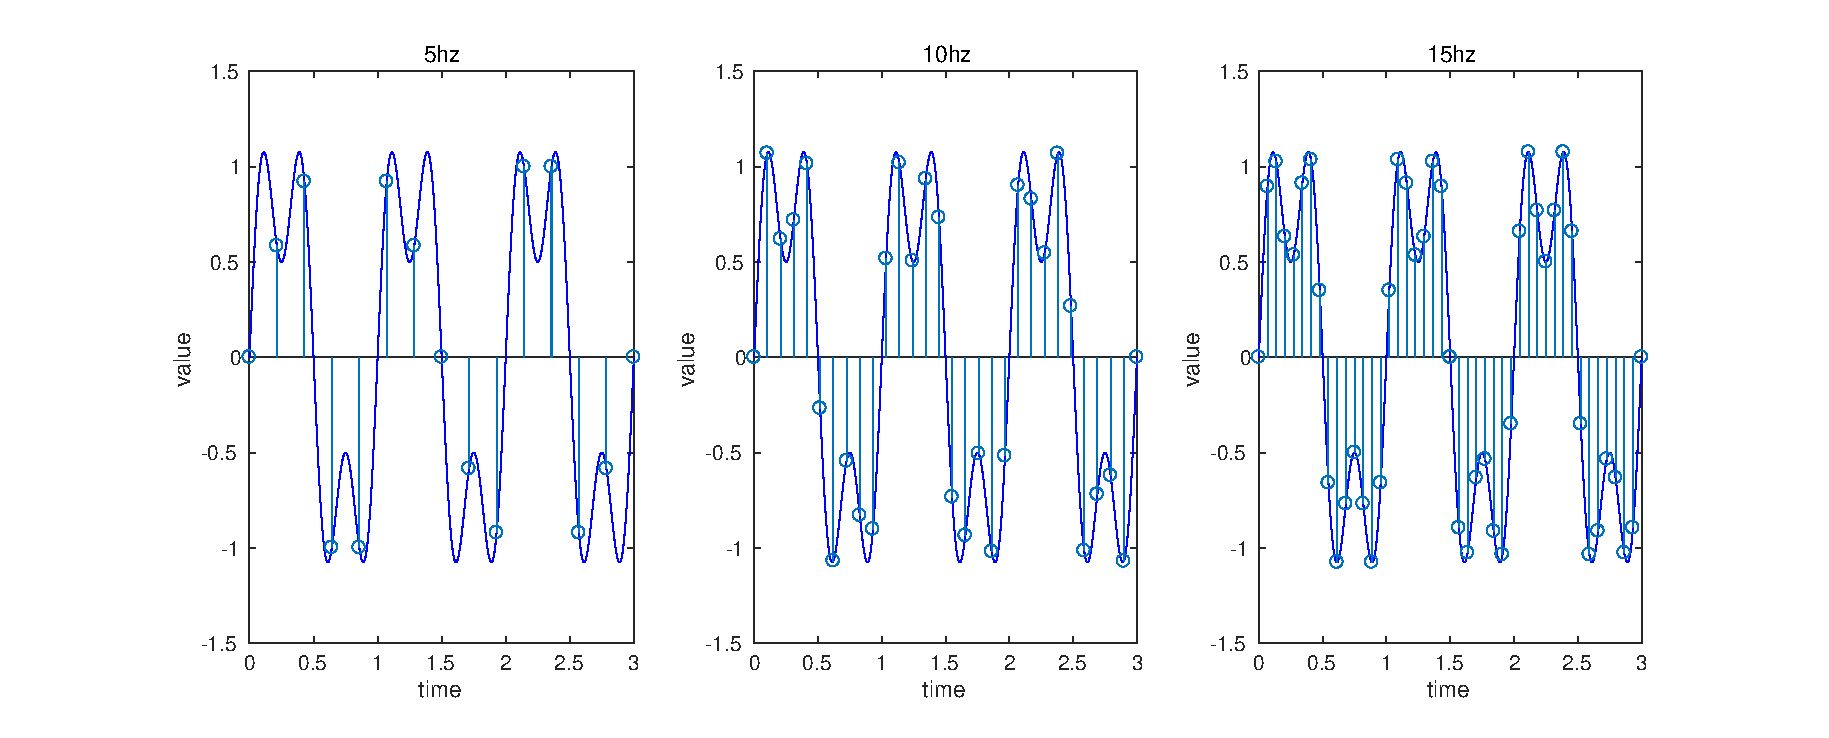
\includegraphics[scale=0.3]{pro2_subpro1.eps}
  \caption{不同采样率所得离散信号图谱}
  \label{pro2_fig1}
\end{figure}


\end{CJK}
\end{document}
